% -*- root: ../GeometriaDiferencial.tex -*-
\chapter{Teorema de Gauss-Bonnet}
\label{chapGaussBonnet}

\section{Introducción y motivación}

El último tema del curso va a tratar de formalizar una idea que ha asomado la cabeza en temas anteriores: la conexión entre la topología y la geometría. Por ejemplo, con el Lema de Poincaré (\ref{thmPoincare}) veíamos que, de algún modo, las formas diferenciales ``veían'' el espacio en el que estaban definidas. La cohomología de De Rham (\ref{defCohomologiaDeRham}) también nos daba pistas de esa relación entre geometría y topología.

La cuestión es que hay una relación todavía más profunda entre ambas. Esta relación es la que se materializa con el teorema de Gauss-Bonnet que vamos a ver ahora. De momento, eso sí, nos quedaremos en superficies, estudiando a lo largo del capítulo la variedad $M$ 2-dimensional, compacta, orientable o Riemanniana.

\section{Índice de un campo}

A lo largo de esta sección vamos a considerar un campo $X$ definido en $M$, y vamos a estudiar sus puntos singulares.

\begin{defn}[Punto\IS singular] Se dice que $p∈M$ es singular si $X(p) = 0$. \end{defn}

Si hay un entorno de $p$ en el que $p$ es el único punto singular, entonces es un punto singular aislado. Dado que hemos pedido que la variedad sea compacta, sabemos que habrá un número finito de puntos aislados.

Algo que nos va a interesar, todavía no sé por qué, es ver cuántas vueltas da nuestro campo $X$ cuando nos movemos rodeando el punto singular.

\begin{defn}[{Í}ndice] Suponemos que $X$ tiene un número finito de puntos singulares aislados. Consideramos entonces en $U\setminus\set{p}$ una referencia dada por \[ \gor{e}_1 ≝ \frac{X}{\md{X}} \] y el vector $\gor{e}_2$ que completa la referencia ortonormal y mantiene la orientación. De esa referencia salen $\gor{ω}_1,\gor{ω}_2, \gor{ω}_{12}$ como las 1-formas duales.

Construimos también una referencia $ω_1, ω_2, ω_{12}$ a partir de coordenadas locales. Así, tenemos otra referencia móvil para estudiar la del gorro, y por lo tanto tendremos la fórmula \[ \gor{ω}_{12} = ω_{12} - τ \] del lema \ref{thmOmegaTau}.

Si tomamos ahora una curva $C$ que encierra el disco con el sentido de giro dado por la orientación. Sabemos entonces que \[ \int_C τ = \int_C \dif φ \] donde $φ$ es el ángulo de la dos referencias que vimos en \ref{eqPhiAngulo}. Esa integral, por ser una curva cerrada, tiene que ser igual a $2πI$, con $I ∈ ℤ$. A esa $I$ se le llama el \textbf{índice} de $X$ en $p$.
\end{defn}

\begin{figure}[hbtp]
\centering
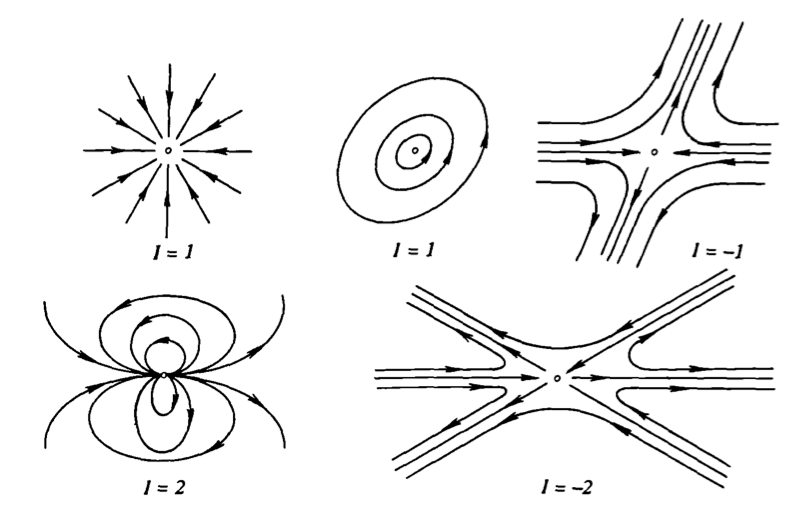
\includegraphics[width=0.8\textwidth]{img/IndiceCampos.png}
\caption{Índice de varios campos. Imagen de \cite[Fig. 6.1, p. 101]{doCarmo94}.}
\label{figIndiceCampos}
\end{figure}

El índice será 1, por ejemplo, si damos una vuelta alrededor del punto en el mismo sentido de la orientación. La imagen \ref{figIndiceCampos} muestra varios posibles campos con sus índices.

Hay que notar que durante la definición hemos hecho varias elecciones: de la curva, de la referencia y de la métrica. Antes de seguir, hemos de demostrar que el índice está efectivamente bien definido.

\begin{lemma} El índice no depende de la curva $C$ escogida siempre que sea topológicamente una circunferencia y contenga únicamente al punto singular $p$.
\end{lemma}

\begin{proof} Si cogemos $I_1, I_2$ los índices dados por dos curvas $C_1, C_2$, vemos que \[ I_1 - I_2 = \frac{1}{2π} \int_{C_1} τ - \frac{1}{2π} \int_{C_2} τ \eqexpl{Stokes} \frac{1}{2π} \int_Δ \dif τ = 0\] donde $Δ$ es la región encerrada entre $C_2$ y $C_1$, ya que $\dif τ = 0$.
\end{proof}

\begin{lemma} El índice no tepende de la referencia tomada $\set{e_1, e_2}$ que nos da las formas $ω_1, ω_2, ω_{12}$.
\end{lemma}

\begin{proof} Consideramos $p$ y una circunferencia estándar $S_r$ en la carta. Suponemos $p = (0,0)$ en la carta. La circunferencia encerrará una bola de radio $r$ $\bola_r$. Calculamos el límite siguiente \( \lim_{r\to 0} \frac{1}{2π} \int_{S_r} \gor{ω}_{12} ≝ \gor{I} \label{eqProofRef1} \)

Además, vamos a tratar de demostrar que $I = \gor{I}$, esto es, que el índice no depende de la referencia tomada $\set{e_1, e_2}$ sino más bien de la referencia $\set{\gor{e}_1, \gor{e}_2}$ que construimos a partir del vector.

Para demostrar que existe el límite, consideramos la sucesión de números reales $\int_{S_{r_i}} \gor{ω}_{12}$ y vemos que es de Cauchy. Evaluamos la diferencia \( \int_{S_{r_1}} \gor{ω}_{12} - \int_{S_{r_2}} \gor{ω}_{12} \eqexpl{Stokes} \int_Δ \dif \gor{ω}_{12} \label{eqProofRef2} \), donde de nuevo $Δ$ es la región encerrada por las dos curvas $S_{r_1}, S_{r_2}$. Cuando hacemos tender $r_1, r_2 \to 0$, es claro que esa integral se va a cero. Luego la sucesión es de Cauchy y el límite existe.

Ahora hay que ver que el límite es igual al índice. Para eso fijamos un $r_1$ y hacemos tender $r_2$ a 0 en \eqref{eqProofRef2} y tenemos que \( \lim_{r_2 \to 0}  \int_{S_{r_1}} \gor{ω}_{12} - \int_{S_{r_2}} \gor{ω}_{12} = \int_{S_{r_1}} \gor{ω}_{12} - 2π\gor{I} \label{eqProofRef3} \) usando \eqref{eqProofRef1} para decir que $\lim_{r_2\to 0} \int_{S_{r_2}} \gor{ω}_{12} = 2π\gor{I}$.

Pero también podemos aplicar Stokes en \eqref{eqProofRef2} y nos queda que
\(
	\lim_{r_2 \to 0}  \int_{S_{r_1}} \gor{ω}_{12} - \int_{S_{r_2}} \gor{ω}_{12} \eqexpl{Stokes}
	\int_{\bola_{r_1}} \dif \gor{ω}_{12} - \lim_{r_2 \to 0} \underbracket{\int_{\bola_{r_2}}\dif \gor{ω}_{12}}_{\to 0} =
	\int_{\bola_{r_1}} \dif \gor{ω}_{12}
	\label{eqProofRef4}
\)

Juntando \eqref{eqProofRef3} y \eqref{eqProofRef4}, nos queda \( \int_{S_{r_1}} \gor{ω}_{12} = \int_{\bola_{r_1}} \dif \gor{ω}_{12} + 2π\gor{I} \label{eqProofRef5} \)

Por otra parte, usando ahora la fórmula del lema \ref{thmOmegaTau} que nos decía que $\gor{ω}_{12} = ω_{12} + τ$, tenemos que \( \int_{S_{r_1}} \gor{ω}_{12} = \int_{S_{r_1}} ω_{12} + \int_{S_{r_1}} τ \eqexpl{Stokes} \int_{\bola_{r_1}} \dif ω_{12} + \int_{S_{r_1}} τ = \int_{\bola_{r_1}} \dif ω_{12}  + 2πI \label{eqProofRef6}\)

Hemos encontrado dos expresiones diferentes para $\int_{S_{r_1}} \gor{ω}_{12}$ en \eqref{eqProofRef5} y \eqref{eqProofRef6}. Si tenemos en cuenta que $\dif τ = 0$, entonces $\dif ω_{12} = \dif \gor{ω}_{12}$. Sólo nos queda rematar: \begin{align*}
\int_{S_{r_1}} \gor{ω}_{12} &= \int_{S_{r_1}} \gor{ω}_{12} \\
\int_{\bola_{r_1}} \dif \gor{ω}_{12} + 2π\gor{I} &= \int_{\bola_{r_1}} \dif ω_{12}  + 2πI \\
2π\gor{I} &= 2πI \\
\gor{I} &= I
\end{align*} y ya tenemos demostrado lo que queríamos\footnote{En \cite[p.101]{doCarmo94} comenta que $\gor{ω}_{12}$ no está definido en todo $\bola_{r_2}$ pero sí que lo está $K \gor{ω}_1 ∧ \gor{ω}_2$, pero no acabo de ver por qué sí puede usar tranquilamente $\gor{ω}_1$. Así que, por no complicarme la vida he dejado ahí $\dif ω_{12}$ sin preocuparme demasiado, supongo que usando cosas parecidas a las de la sección \ref{secIndependenciaEcsEstructura} se podrá llegar a algo que esté bien definido.}.
\end{proof}

\begin{lemma} El índice no depende de la métrica Riemanniana escogida.
\end{lemma}

\begin{proof} Para esta demostración vamos a hacer un truco que es una demostración de la métrica. Definimos dos métricas $\pesc{·,·}_1$, $\pesc{·,·}_2$. Tomamos entonces el segmento que une ambas métricas, cosa que podemos hacer porque las métricas son un espacio vectorial de tensores. Definimos entonces  \[ \pesc{·,·}_t = t \pesc{·,·}_1 + (1-t)\pesc{·,·}_2 \] con $t∈[0,1]$

Es fácil ver que $\pesc{·,·}_t$ es Riemanniana si las dos de antes son Riemannianas. Definimos entonces índices $I_t, I_1, I_2$ con respecto a cada métrica respectivamente.

Por el lema anterior, es fácil ver que $I_t$ va a depender continuamente de $t$. Ahora la conclusión es inmediata: si $I_t$ es continua y valora en los enteros, sólo puede ser constante.
\end{proof}

El teorema de Gauss-Bonet lo que dice es que en una superficie en las mismas condiciones que estábamos viendo antes tenemos una función de curvatura que podemos integrar multiplicada por $σ$ (la 2-forma de área). Pues bien, eso debería dar un invariante de la superficie. Lo que dice Gauss-Bonet es que eso es la suma de los índices de un campo $X$ cualquiera con singularidades aisladas. La fórmula tiene varios aspectos interesantes: el lado izquierdo no depende de $X$ luego no depende del campo.

El sobrino del hombre este tiene dos coronillas y lleva el teorema de Gauss Bonet en la cabeza. Que nosqué de lo de la bola de pelo que no se puede peinar que ya vimos en topología\footnote{Lo de ``vimos'' es un decir.}.

Además, la integral de la curvatura no va a depender de la métrica porque los índices no dependían de la métrica. Además, veremos que eso es un invariante puramente topológico, que eso es la característica $χ(M)$ de Poincaré.


\begin{theorem}[Teorema\IS de Gauss-Bonnet] Sea $M$ una variedad diferenciable de dimensión dos, compacta y orientable. Sea $X$ un campo vectorial diferenciable con singularidades aisladas $p_1, \dotsc, p_k$. Entonces, para cualquier métrica Riemanniana en $M$, se tiene que
\[\frac{1}{2π} \int_M K ω_1 ∧ ω_2 = \sum_{p_i} I_{p_i}(X)\]
con $K$ la curvatura gaussiana.
\end{theorem}

\begin{proof}

El teorema tiene 2 igualdades. Vamos a demostrar la primera con un argumento muy muy parecido al teorema de los residuos.
\[\int_{M-∪B_i} K\bar{ω_1} ∧ \bar{ω_2} \overset{defK}{=} -\int d\bar{ω_{12}} = \overset{St} = \int_{∪dB_i}\bar{ω_{12}} = \sum \int_{dB_i} \bar{ω_R} \]

y lo ha borrado antes de que me diera tiempo a enterarme.


\end{proof}
Para demostrar la segunda igualdad, necesitamos definir un par de cosas.



\begin{defn}[Triangulación]  $M=∪T_i$, siendo $T_i$ una cosa homeomorfa a un triángulo, es decir, con 3 vértices, 3 lados y una cara.

Una triangulación tiene que cumplir la siguiente condición:
\[
T_i ∩ T_j = \begin{cases}
ø\\
lado\\
vétice\\
\end{cases}
\]
\end{defn}


\begin{defn}[Característica Euler-Poincaré]
Sea $M$ una variedad diferenciable,

$$X_τ(M) := \#V - \#L + \#C ∈ℤ$$

Siendo $V$ el número de vértices de una triangulación, $L$ el número de lados y $C$ el número de caras.


Esta característica es una propiedad topológica de la variedad.
\end{defn}

Lo interesante de esta cosa es que no depende de la triangulación elegida, sino de la topología.

Vamos a ver un par de ejemplos:

\begin{example}
Sea $M$ un tetraedro. Tenemos entonces $V=6,A=12,C=8$, con lo que la característica es $2$. Con esto, tenemos (si de verdad fuera topológico, que no lo hemos demostrado todavía) tendríamos que la característica de EP de la esfera es 2 (porque son ¿homeomorfos? el tetraedro y la esfera)
\end{example}

\begin{example}

Vamos a ver la triangulación de un toro. Para ello, es pensamos en el toro como un cuadrado con los lados identificados. Construimos en ese cuadrado un triángulo rectángulo en una esquina y tiramos 4 paralelas a esa, de tal forma que la tercera sea la diagonal.

Así, tenemos $V=9$, $L=27$ y $C=18$. Para calcularlo tenemos que tener cuidado con las identificaciones (cada lado del cuadrado se identifica con el paralelo).
\end{example}


\begin{theorem}[Poincaré]
Sea $D$ un campo en $M$ una variedad
\[
\sum I_i(D) = \mathcal{X}(M) = \#V - \#L + \#C
\]

\end{theorem}

Por el teorema de Gauss Bonnet sabemos que la suma de los índices no depende del campo elegido. Eso es lo que nos va a dar la clave para que no dependa de la triangulación.

\begin{proof}
Esta demostración merece la pena mirarla en el doCarmo (Página 101) que hay unos dibujos de campos que se utilizan en la demostración de verdad al final de la página 103.

El esquema es probar que para toda tirangulación se puede conseguir un campo que cumpla la fórmula.

Una vez tenemos ese campo construido (Fig 6.2 del doCarmo - página 104), por el teorema de Gauss Bonnet, sabemos que la suma de los índices no depende del campo elegido.

\end{proof}

\begin{theorem}[Gauss-Bonnet-Poincaré]
Sea
\[\frac{1}{2π} \int_M Kσ = \sum_{p_i} I_{p_i}(x) = \mathcal{X}(M)\]
\end{theorem}

Aquí finaliza el curso. Nos hemos dejado el último punto del teorema que es la extensión a dimensiones infinitas de la referencia móvil, que es para lo que servía el álgebra multilineal.

Rafa se comenta que ahora siendo los cursos de 3 horas, hay asignaturas  que se quedan cojas. Nos pone el ejemplo de la teoría de Galois, que siendo sólo de 3 horas se queda corta y coja porque no se ven los teoremas realmente interesantes.

